\documentclass[runningheads,a4paper]{llncs}

\usepackage{amssymb}
\setcounter{tocdepth}{3}
\usepackage{graphicx}
\usepackage{subfig}
%\linespread{2}

\usepackage{url}
\usepackage{csquotes}
\newcommand{\keywords}[1]{\par\addvspace\baselineskip
\noindent\keywordname\enspace\ignorespaces#1}

\usepackage{listings}
\usepackage{color}
\usepackage{enumitem}
\usepackage{hyperref}

\definecolor{dkgreen}{rgb}{0,0.6,0}
\definecolor{gray}{rgb}{0.5,0.5,0.5}
\definecolor{mauve}{rgb}{0.58,0,0.82}

\lstset{frame=tb,
  language=C++,
  aboveskip=3mm,
  belowskip=3mm,
  showstringspaces=false,
  columns=flexible,
  basicstyle={\small\ttfamily},
  numbers=left,
  numberstyle=\tiny\color{gray},
  keywordstyle=\color{blue},
  morekeywords={vector},
  commentstyle=\color{dkgreen},
  stringstyle=\color{mauve},
  breaklines=true,
  breakatwhitespace=true,
  tabsize=3
}

\begin{document}

\mainmatter  % start of an individual contribution

% first the title is needed
\title{Menura: \\ Realtime pitch detection in C++}

% a short form should be given in case it is too long for the running head
\titlerunning{menura}

%
\author{Valentina Visintini}
%
\authorrunning{menura}
% (feature abused for this document to repeat the title also on left hand pages)

\institute{Practical Course "Advanced Software Development with Modern C++"\\Summer Term 2018\\Institute for Computer Science\\
Ludwig-Maximilians-Universit\"at M\"unchen\\
}

\maketitle


\section{Introduction}
A typical task of digital signal processing is to identify the pitch of an audio signal. To achieve this in realtime, C++ ...


\section{A Brief Outline of Acoustics}
In music, a \textit{pitch} is the position of a single sound within the complete range of sound, which is perceived according to the frequency of vibration of the sound waves. Human listeners perceive higher frequencies as higher pitches, hence a lower pitch is indicative of a lower frequency.
A pitch detector aims to find the fundamental frequency of an audio signal, i. e. the lowest frequency of a periodic waveform, to determine what note is being played. Since the fundamental is also perceived as the loudest, the ear identifies it as the specific pitch of the musical tone

Sound waves cause a local pressure deviation from the ambient atmospheric pressure, which is known as sound pressure and perceived as \textit{loudness}. Even though it can be ordered on a scale extending from quiet to loud, loudness cannot be measured objectively, as its perception changes individually, whereas the actual sound pressure can be measured using a microphone and expressed in decibel (dB). The sound pressure level $L_p$ is defined by a logarithmic measure of the effective pressure of a sound $p$ relative to the standard reference sound pressure $p_0$ in air or water. 

\begin{equation}
L_p = 20 * \log_{10}(\frac{p}{p_0}) \mathrm{dB}
\label{eq:spl}
\end{equation}

\section{Frequency Spectrum Analysis}
The fundamental frequency of an audio signal can be obtained by a fast Fourier transform (FFT). This algorithm samples a signal over a period of time and divides it into its frequency components, converting it from the time domain to a representation in the frequency domain.

\begin{equation}
\sum_{n=0}^{N-1}x_n  e^{-i 2 \pi k\sqrt{-1}/N}
\label{eq:fft}
\end{equation}

In order to detect the pitches of an audio signal, it is split up in equal sample windows and each window is analyzed separatedly. The size of the windows, i. e. the FFT size, affects the resolution of the resulting spectra: the larger the size, the higher it is.
The resulting output is divided into bins which contain the magnitude information for the respective frequency.

The magnitude of each FFT bin i can be expressed like this:
\begin{equation}
mag(i) = \sqrt{(re(i)^{2} + im(i)^{2})}
\label{eq:mag}
\end{equation}

To obtain the loudness of each frequency, the magnitude must be transformed to decibel:

\begin{equation}
A(i) = 20 * \log_{10}( mag(i) ) \mathrm{dB}
\label{eq:loc}
\end{equation}

Starting from this, the frequency with the largest magnitude can be identified as the fundamental frequency of the analyzed window.


\section{Modeling}
To realize a pitch detector, an audio signal must be converted to a sequence of samples first. 

 

\begin{figure}[]
  \centering
  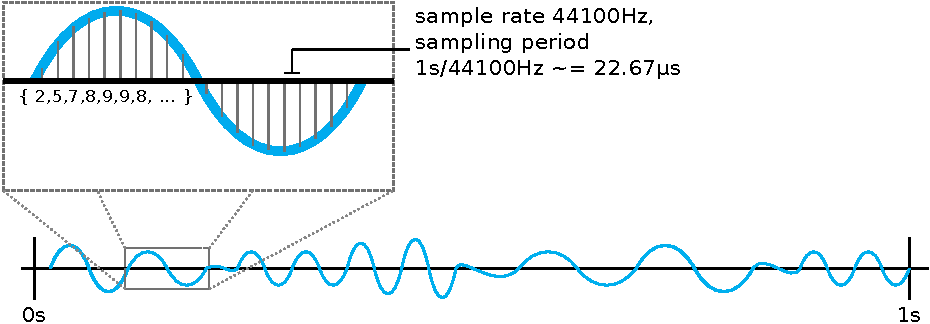
\includegraphics[width=\textwidth]{img/menura_sampling.pdf}
  \caption{Audio sampling}
  \label{fig:sample2}
\end{figure}


\textbf{
\begin{figure}[]
  \centering
  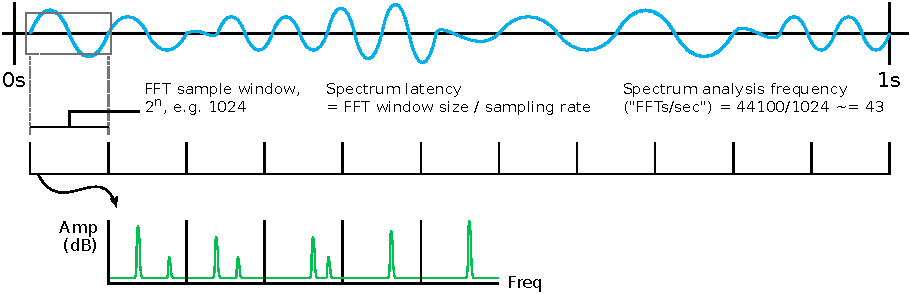
\includegraphics[width=\textwidth]{img/menura_fft.pdf}
  \caption{Frequency Spectrum Analysis \& Signal Transformation: Time Domain to Frequency Domain}
  \label{fig:fft}
\end{figure}
}

\textbf{
\begin{figure}[]
  \centering
  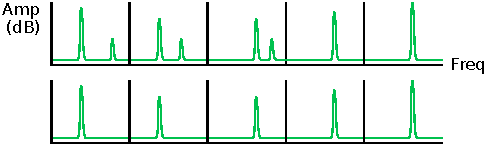
\includegraphics[width=0.5\textwidth]{img/menura_pruning.pdf}
  \caption{Pruning}
  \label{fig:prune}
\end{figure}
}

\textbf{
\begin{figure}[]
  \centering
  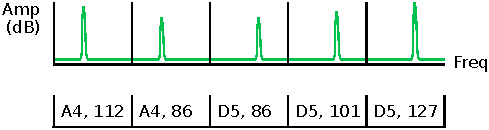
\includegraphics[width=0.5\textwidth]{img/menura_note.pdf}
  \caption{Classification}
  \label{fig:class}
\end{figure}
}

Find corresponding key on piano:
\begin{equation}
n = 1200 \cdot \log_2 \left( \frac{b}{a} \right)
\end{equation}


Calculate deviation:
\begin{equation}
d_f = 49 + 12  \cdot \log_2 \left(\frac {f}{440\ \mathrm{Hz}}\right)\,
\end{equation}

\section{Implementation}

\textbf{
\begin{figure}[]
  \centering
  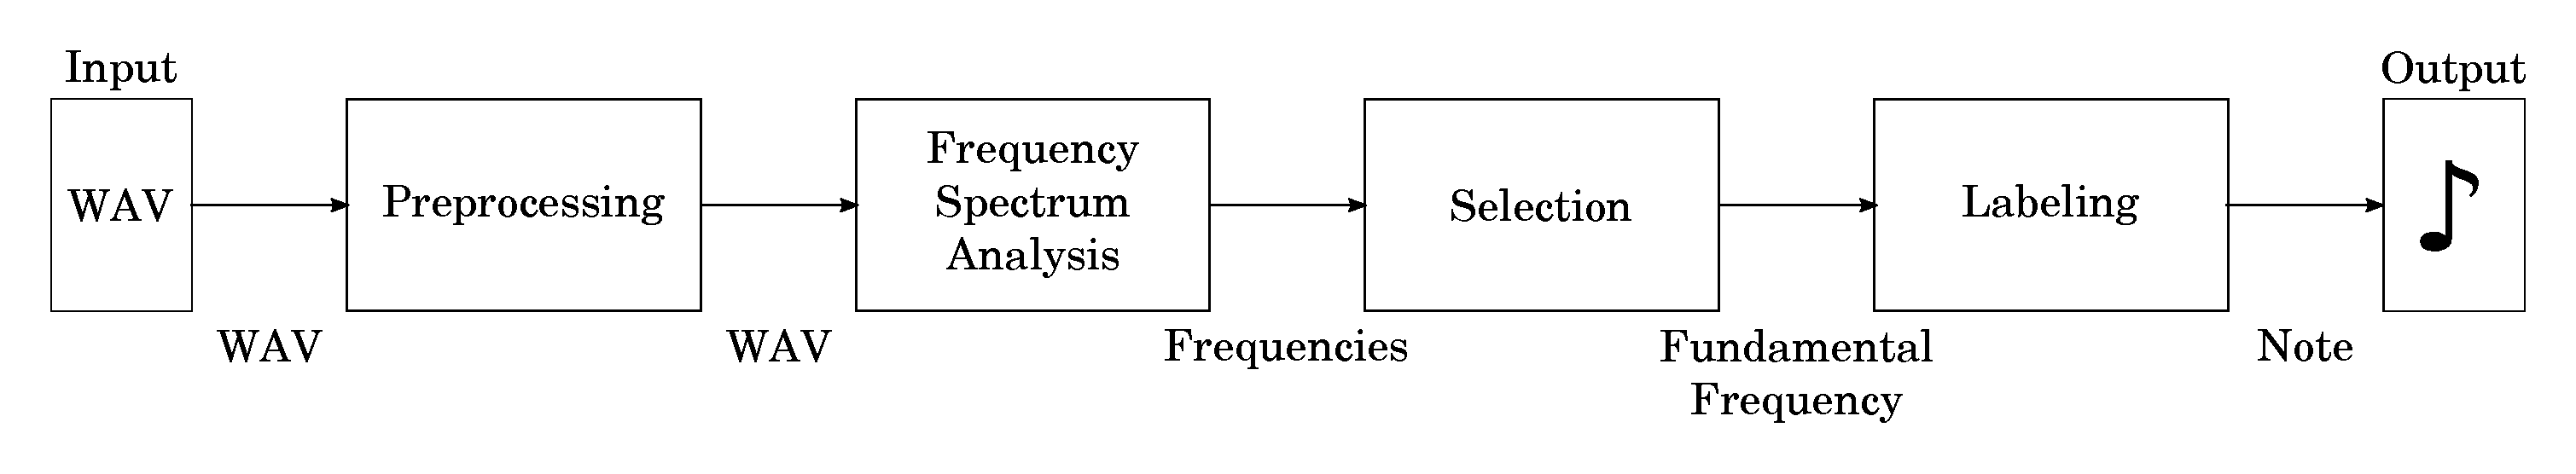
\includegraphics[width=\textwidth]{img/systemdiagram.pdf}
  \caption{System diagram}
  \label{fig:sysdia}
\end{figure}
}





\bibliography{literature}
\bibliographystyle{plain}

\end{document}
